\chapter{Results}
//TODO: Write better intro to chapter, maybe put video link in introduction?

This chapter will present the results of the project. The physical result is depicted i Figure \ref{fig:board-top}.
A video clip of the tunnel program in Appendix \ref{app:tunnel} is available at \href{https://vid.me/JEZv}{https://vid.me/JEZv} \cite{tunnel-demo}.

\begin{figure}[h!]
	    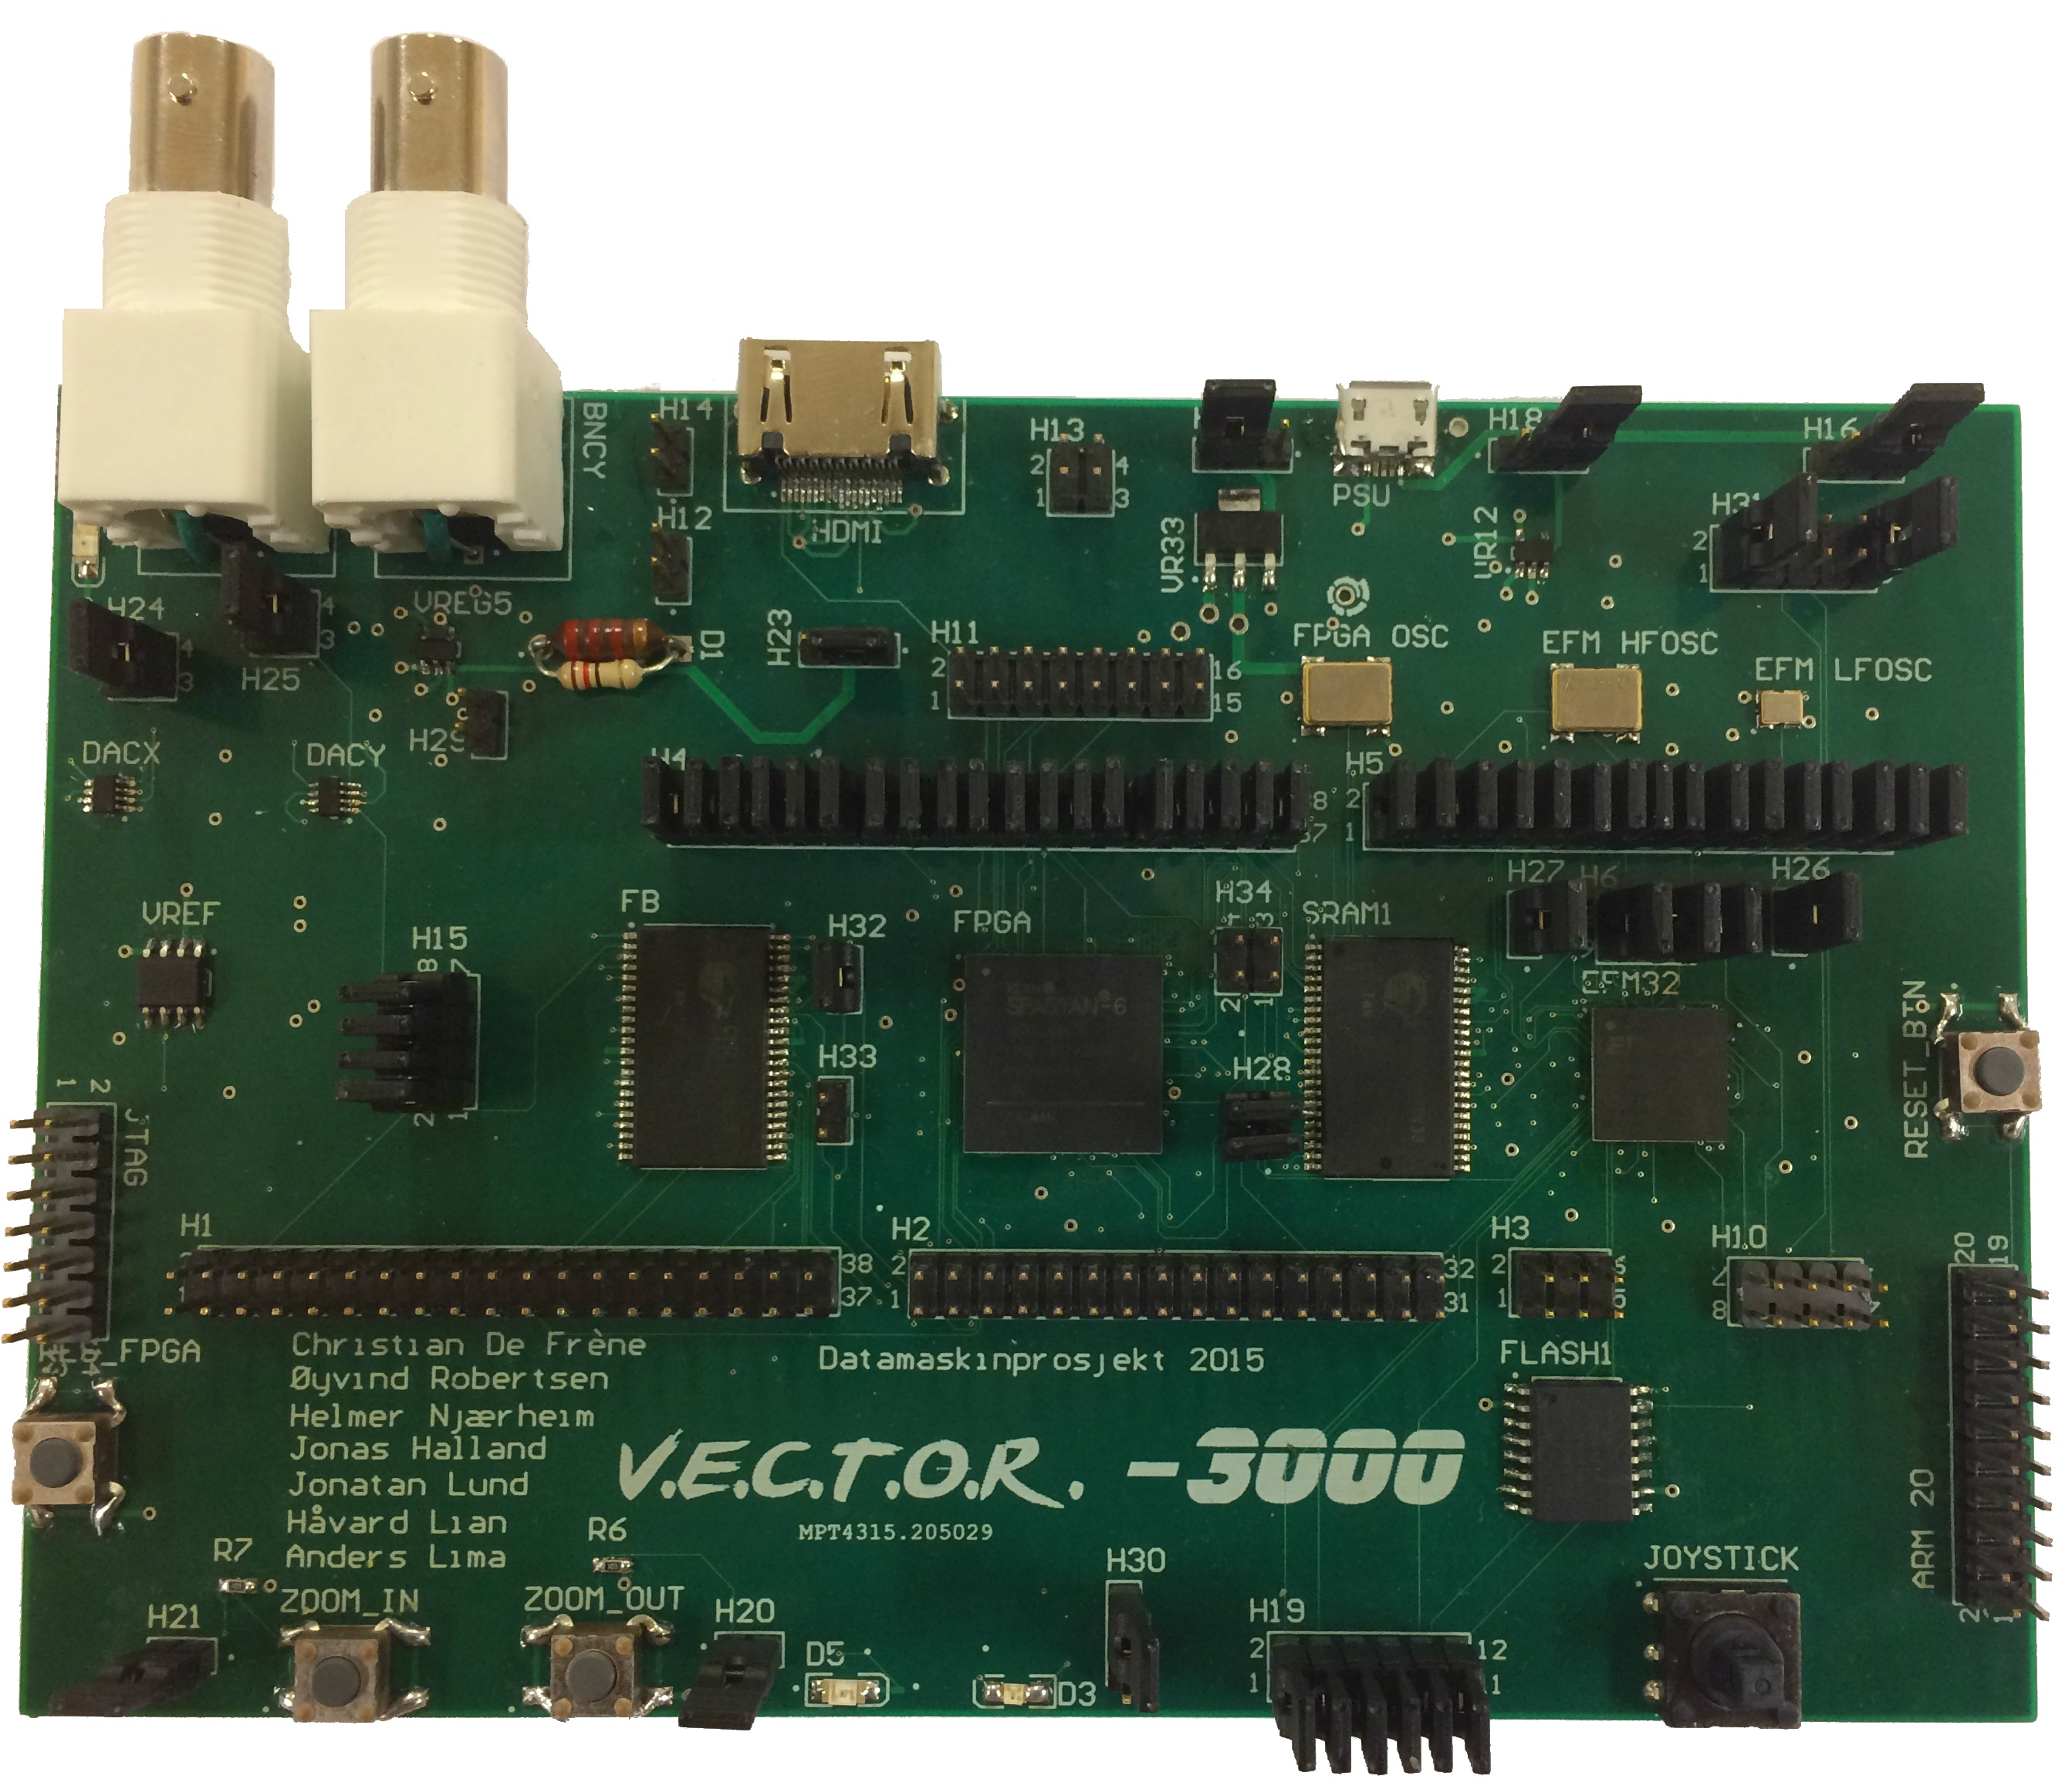
\includegraphics[width=\linewidth]{images/board_top.jpg}
	    \caption{An image of the finished \vthreek board}
	    \label{fig:board-top}
\end{figure}

\section{Storage}
The final implementation utilizes BRAM to achieve highest possible clock frequency and avoid unnecessary SRAM access delays.
With the current implementation the BRAM can hold a total of 1024 primitives.
The synthesis report from Xilinx Ise states that the FPGA still has more BRAM after.
However the primitive storage space is not the limiting factor, but the primitive drawing module.

\section{Performance}
The maximum clock frequency of the DACs is 30MHz according to the datasheet.
To update the DAC value a total of 25 clock cycles are required.
As a result the theoretical effective maximum output will be \(30 MHz \div 25 = 1.2 MHz \).
However during testing the group experience incorrect DAC values if the clock were set higher than 20 MHz.
With a clock frequency of 20 MHz the maximum output is 800 KHz.

\section{Video Output}
\vthreek was successful in drawing primitives to the a screen.
Only one of the output modules were realized; the analogue oscilloscope output.

\subsection{Oscilloscope}
In Figure \ref{fig:square}, one can see great improvement in the accuracy when drawing a square, compared to the result in Figure \ref{fig:osc_poc}.

\begin{figure}[h!]
	    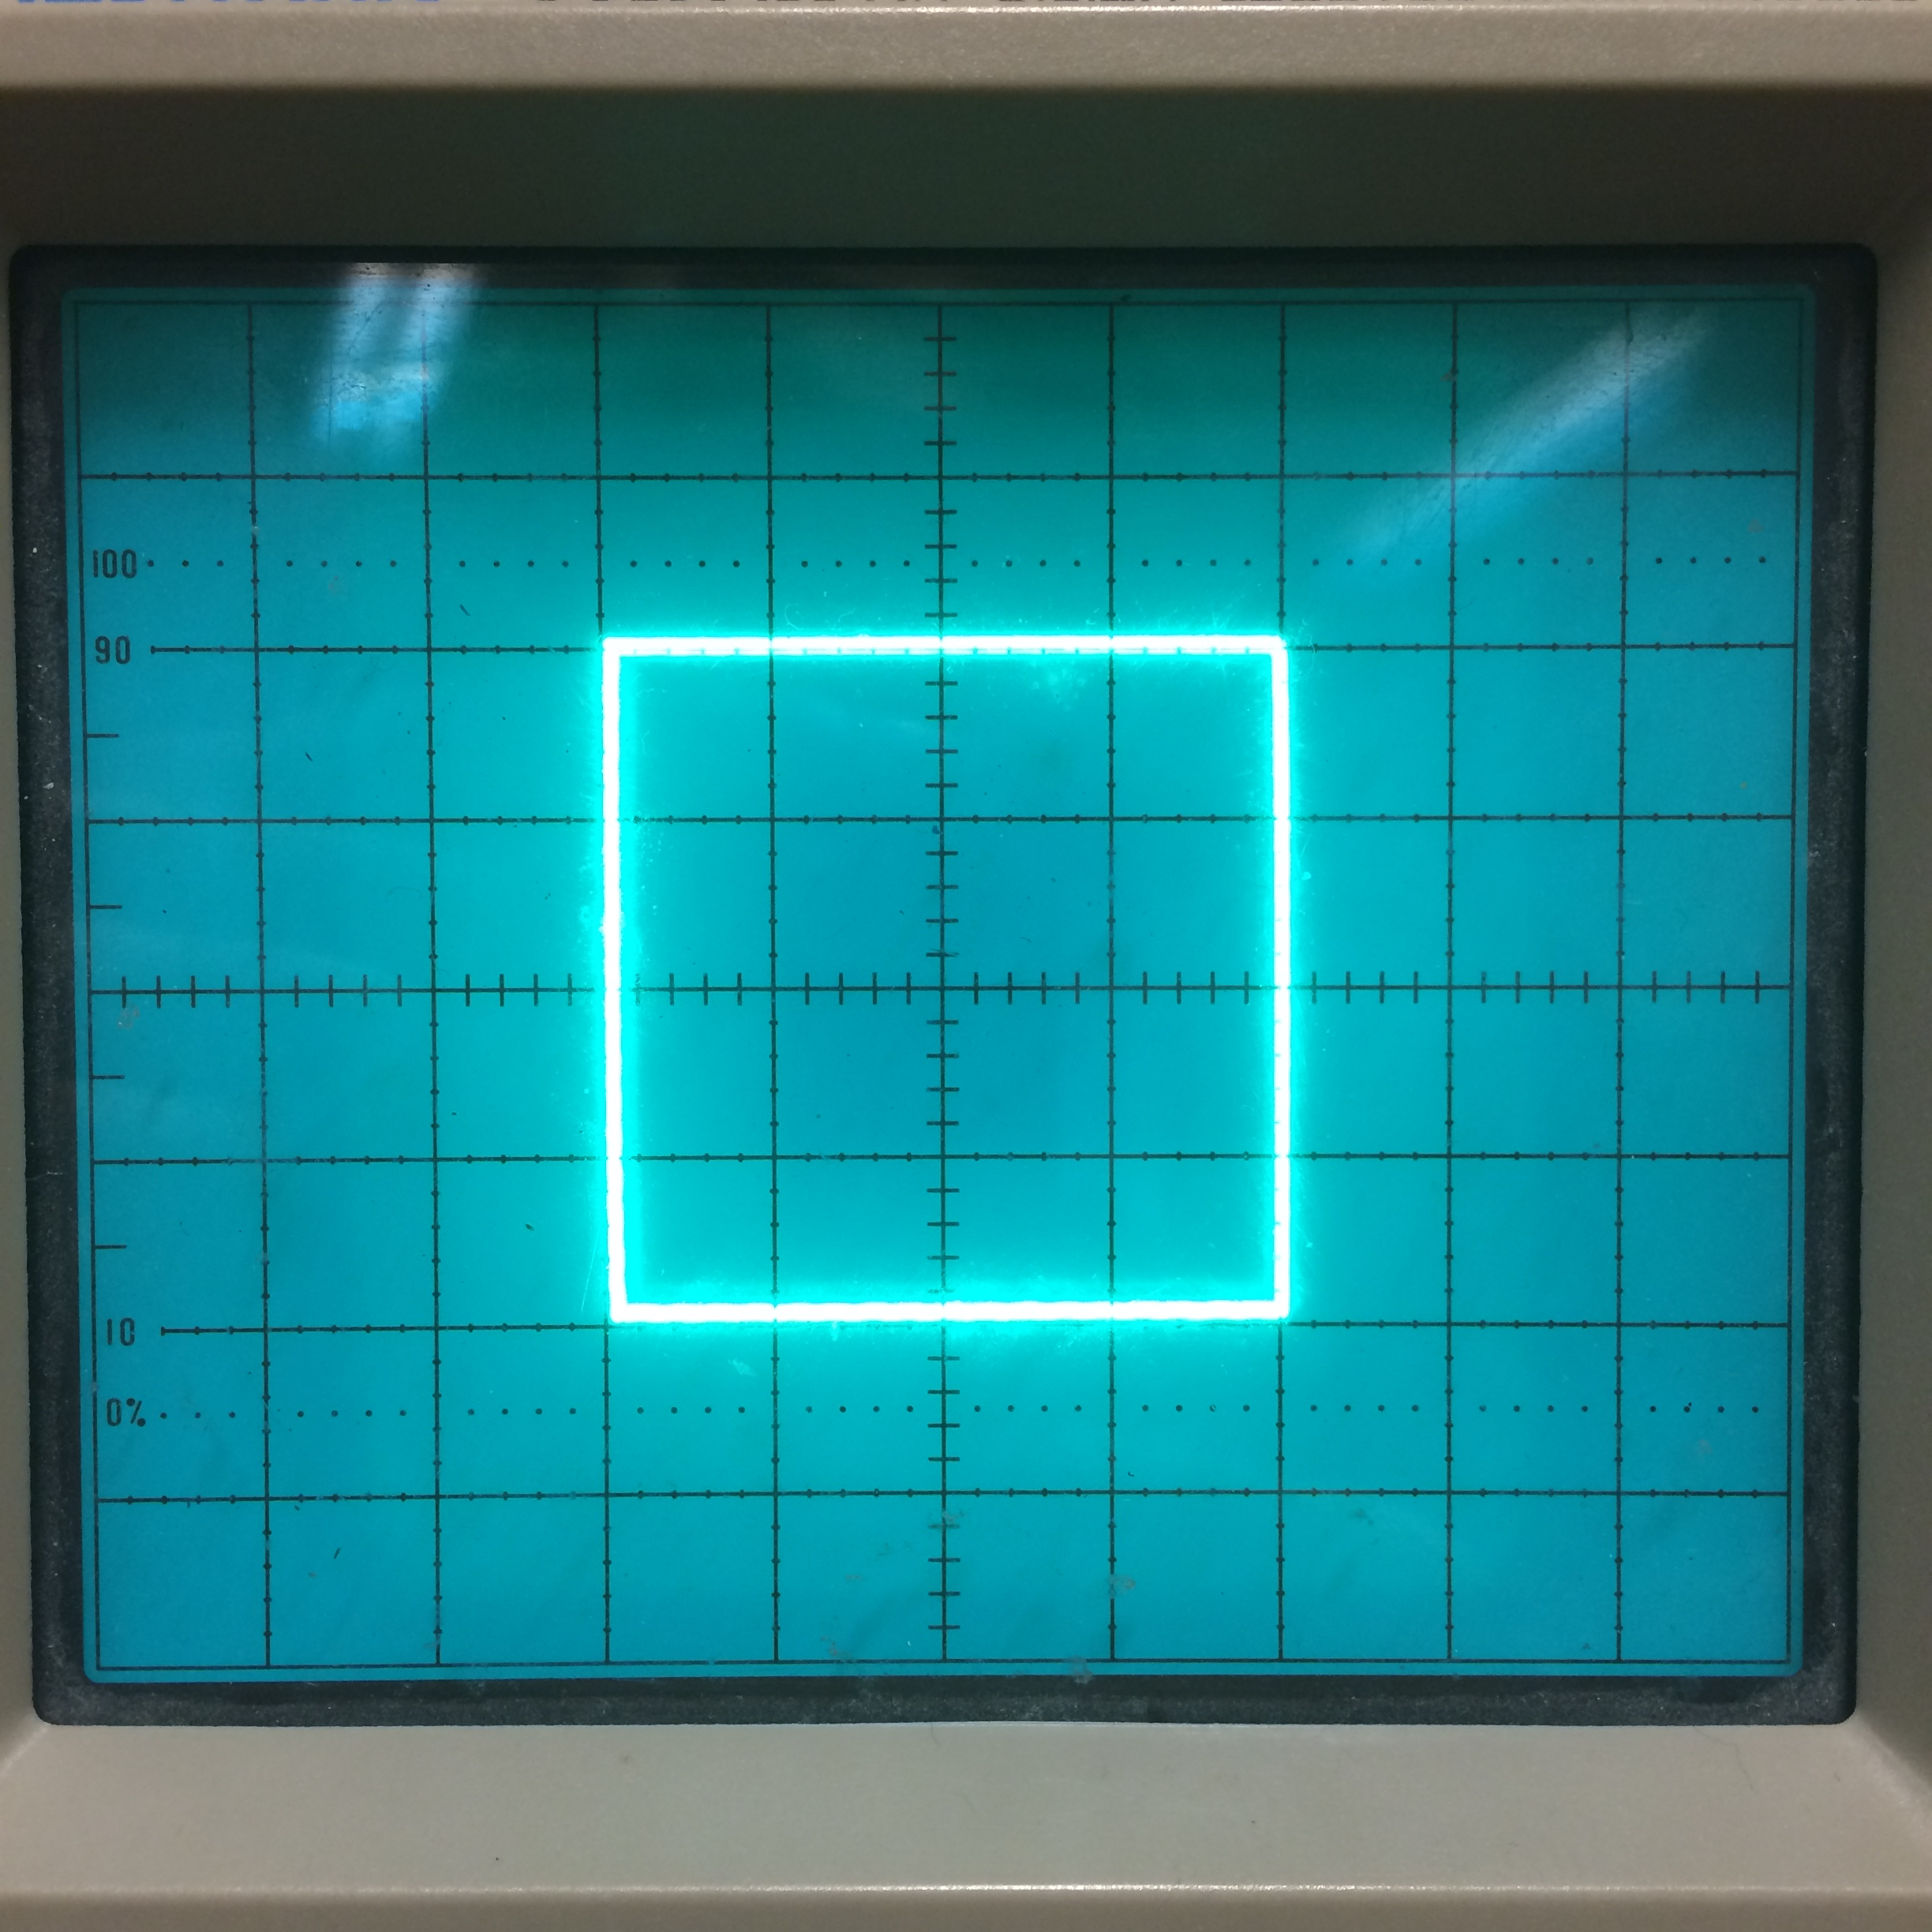
\includegraphics[width=\linewidth]{images/square.jpg}
	    \caption{A square drawn with the finished implementation}
	    \label{fig:square}
\end{figure}


\subsubsection{Drawing Artefacts}
\label{results:artefacts}
Even though drawing to the oscilloscope looks nice, some artefacts were discovered.
This Section will show, and explain two of them.

When the oscilloscope is done drawing one primitive and moves to the next the electron beam i still drawing,
and weaker drawing lines may be visible.
In other words all shapes are drawn without "lifting the pencil off the paper".
If one take a closer look at Figure \ref{fig:artefact}, the drawing artefacts are visible.
There are solutions to avoid the drawing artefacts, which is explained in section \ref{discussion:artefacts}.

\begin{figure}[h!]
	    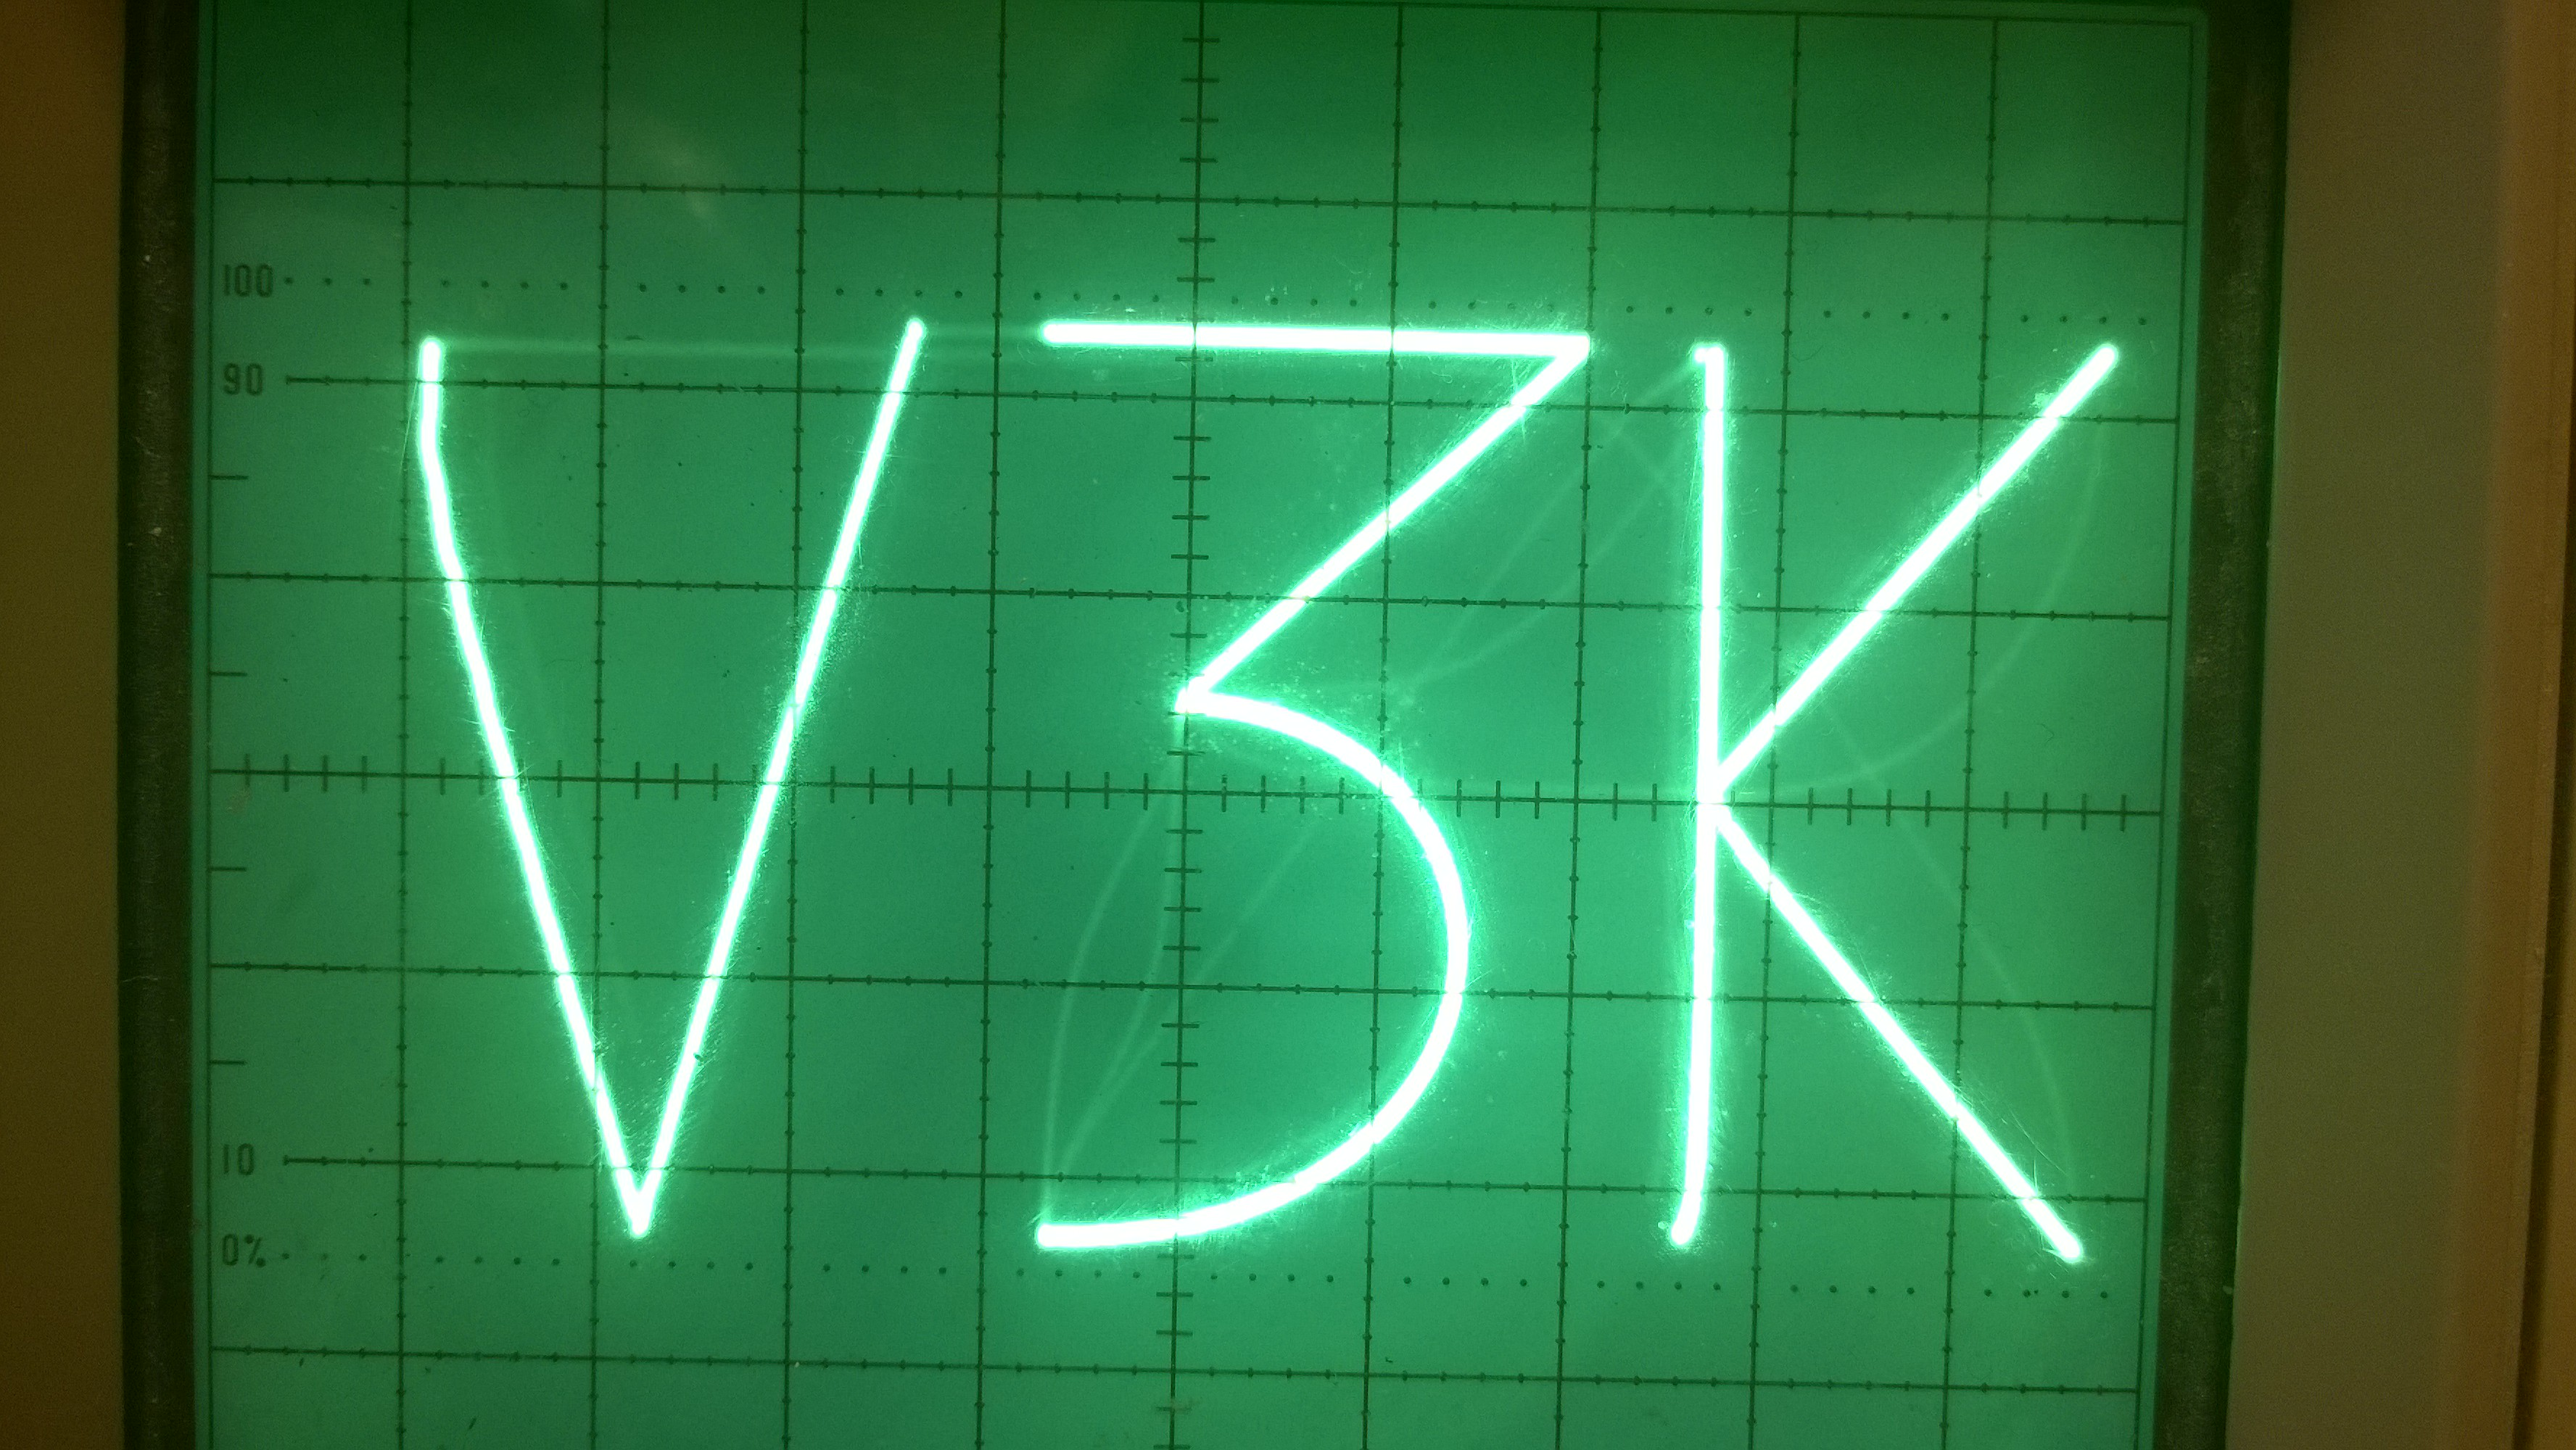
\includegraphics[width=\linewidth]{images/artefacts.jpg}
	    \caption{Drawing V3K with artefacts}
	    \label{fig:artefact}
\end{figure}

Another artefact, also barely visible, is the dots that each primitive is made of.
By zooming in on the oscilloscope this becomes more visible, and can be seen in Figure \ref{fig:artefact-dots}.
The digital nature of \vthreek implies a discrete increments when drawing.
The electron ray moves faster then the DACs are able to feed it with new data.
As a result, the ray will wait at one spot, until it receives new values.
This results in dotted lines, shown in Figure \ref{fig:dotx4} and \ref{fig:dotx8}

\begin{figure}[h!]
   	\centering
    \begin{subfigure}[b]{\textwidth}
   		\centering
       	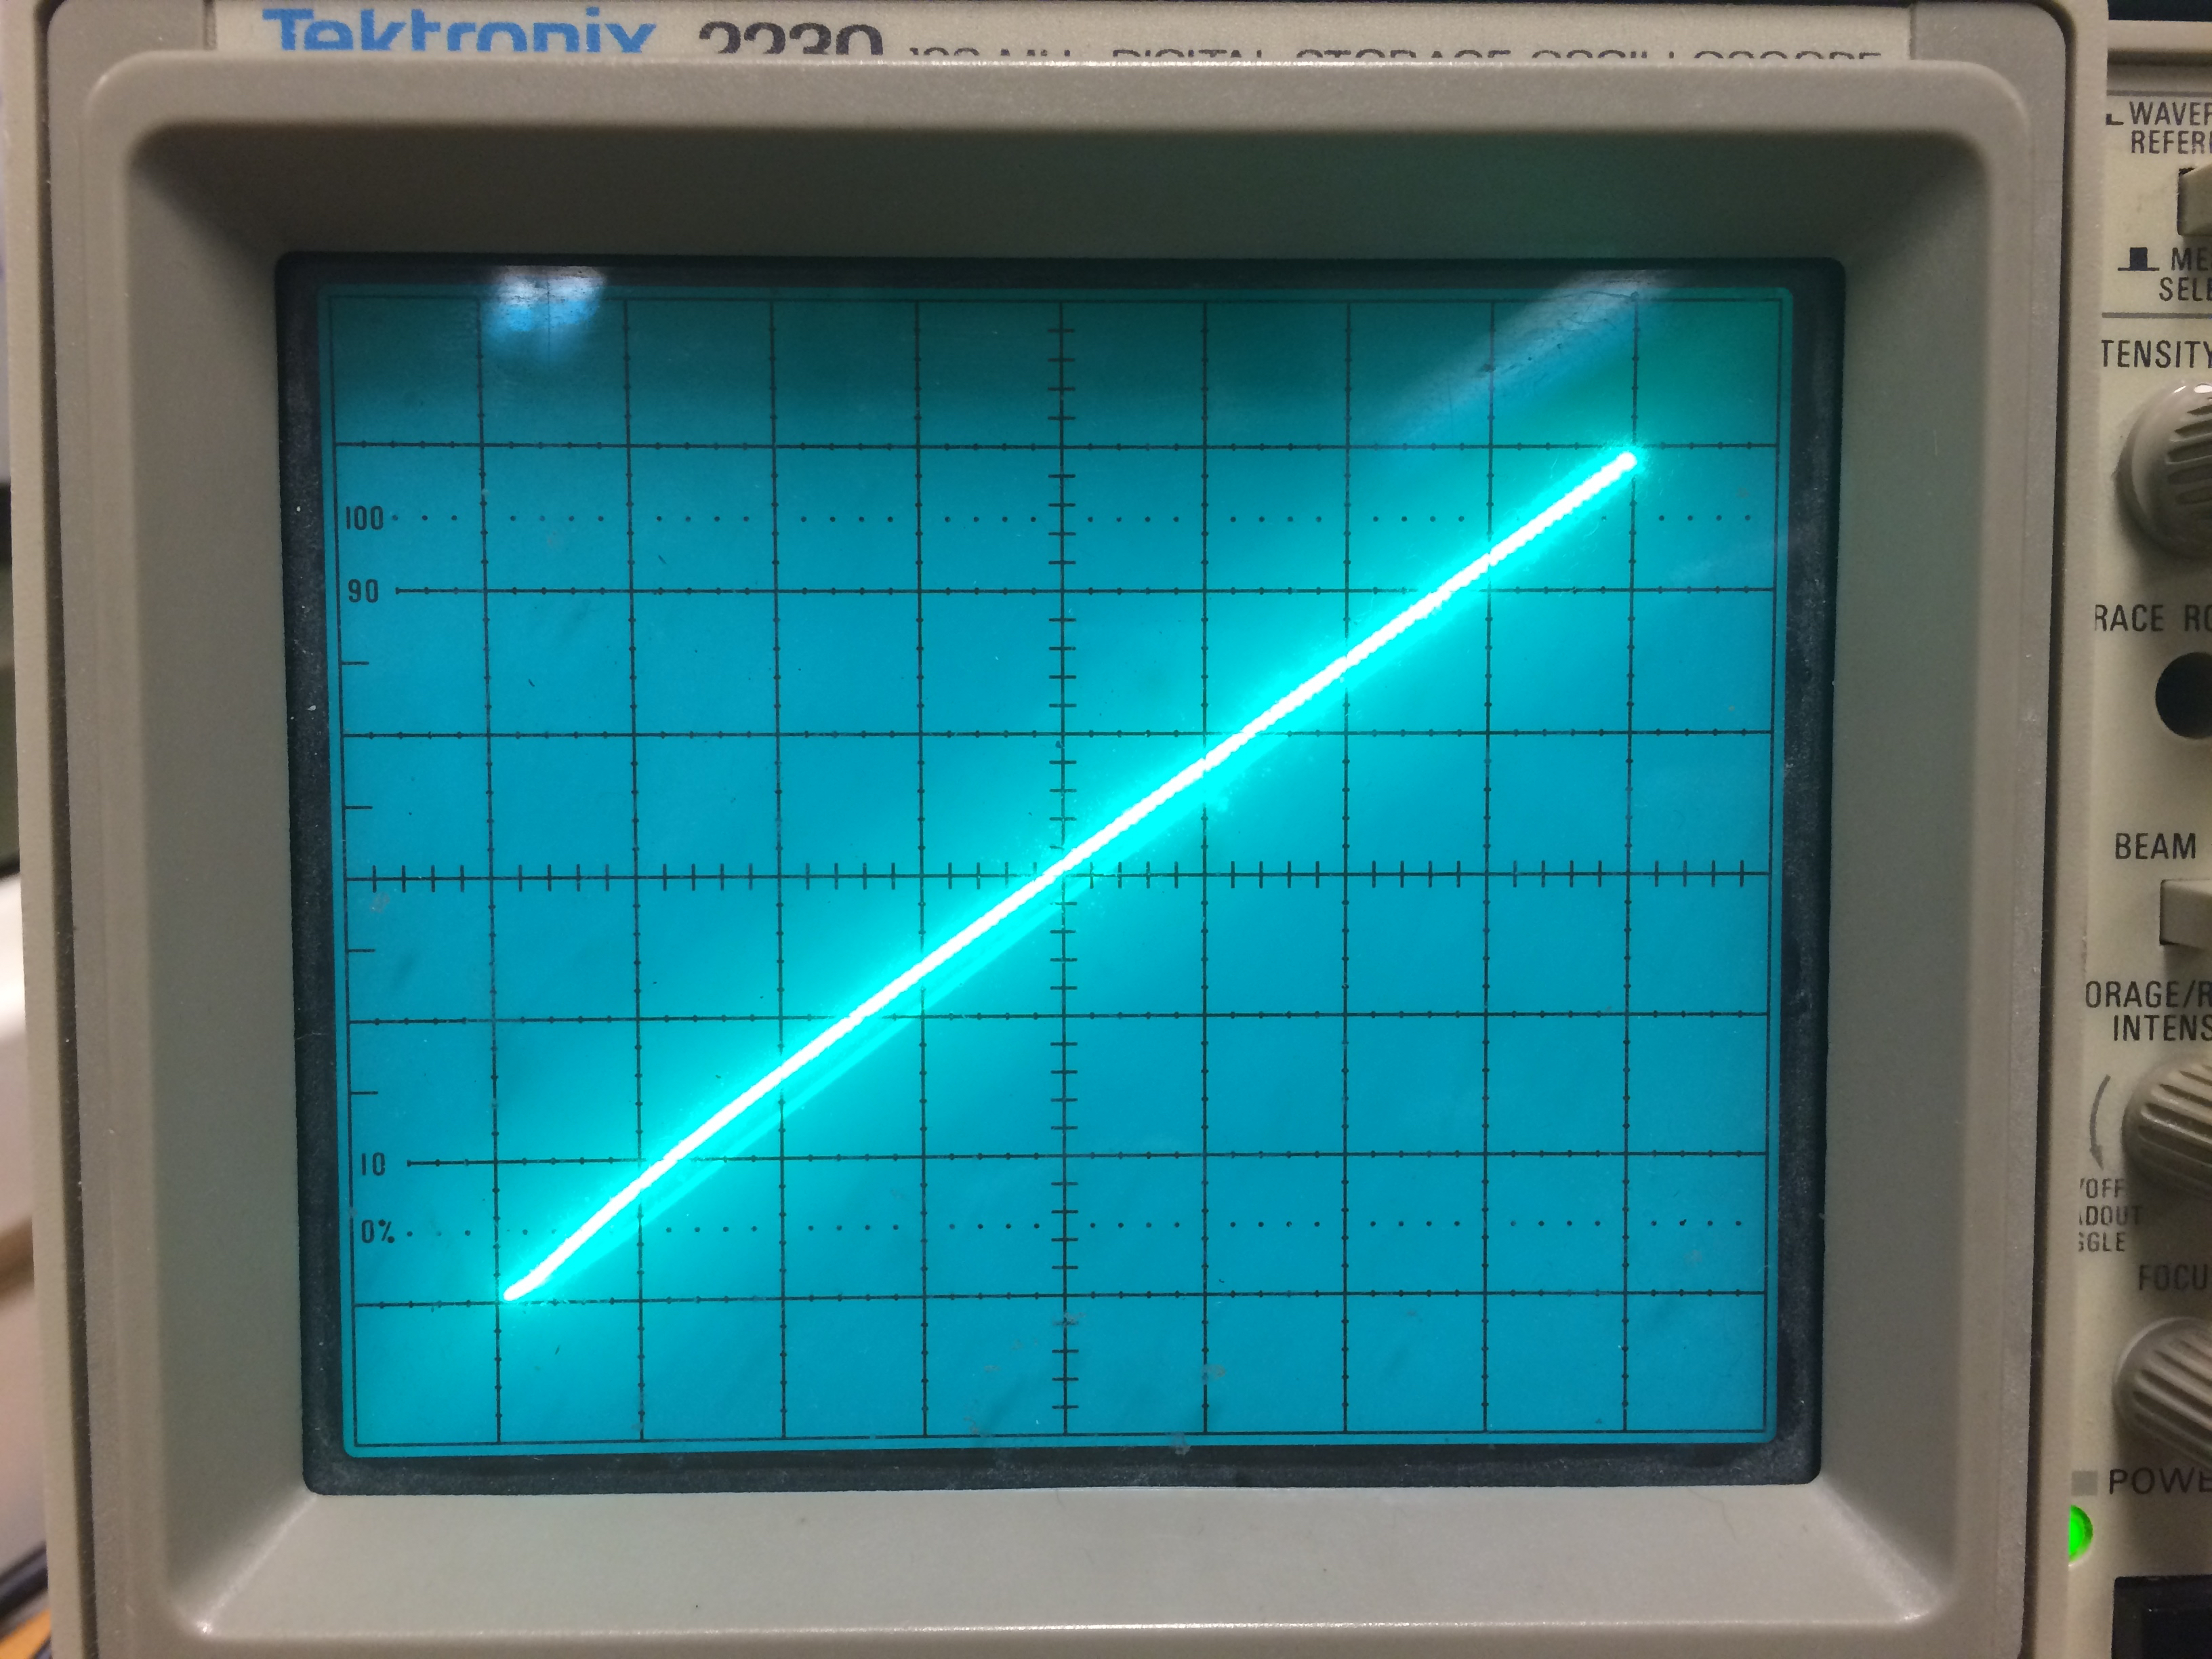
\includegraphics[height=0.4\textheight]{images/dots_x1.jpg}
       	\caption{Dot artefact close to invisible.}
       	\label{fig:dotx1}
    \end{subfigure}
\end{figure}

\begin{figure}[h!]
	\ContinuedFloat
    \begin{subfigure}[b]{\textwidth}
		\centering        
        \includegraphics[height=0.4\textheight]{images/dots_x4.jpg}
        \caption{Dot artefact becomes more visible when zoomed in four times.}
        \label{fig:dotx4}
    \end{subfigure}
    
    \begin{subfigure}[b]{\textwidth}
		\centering        
        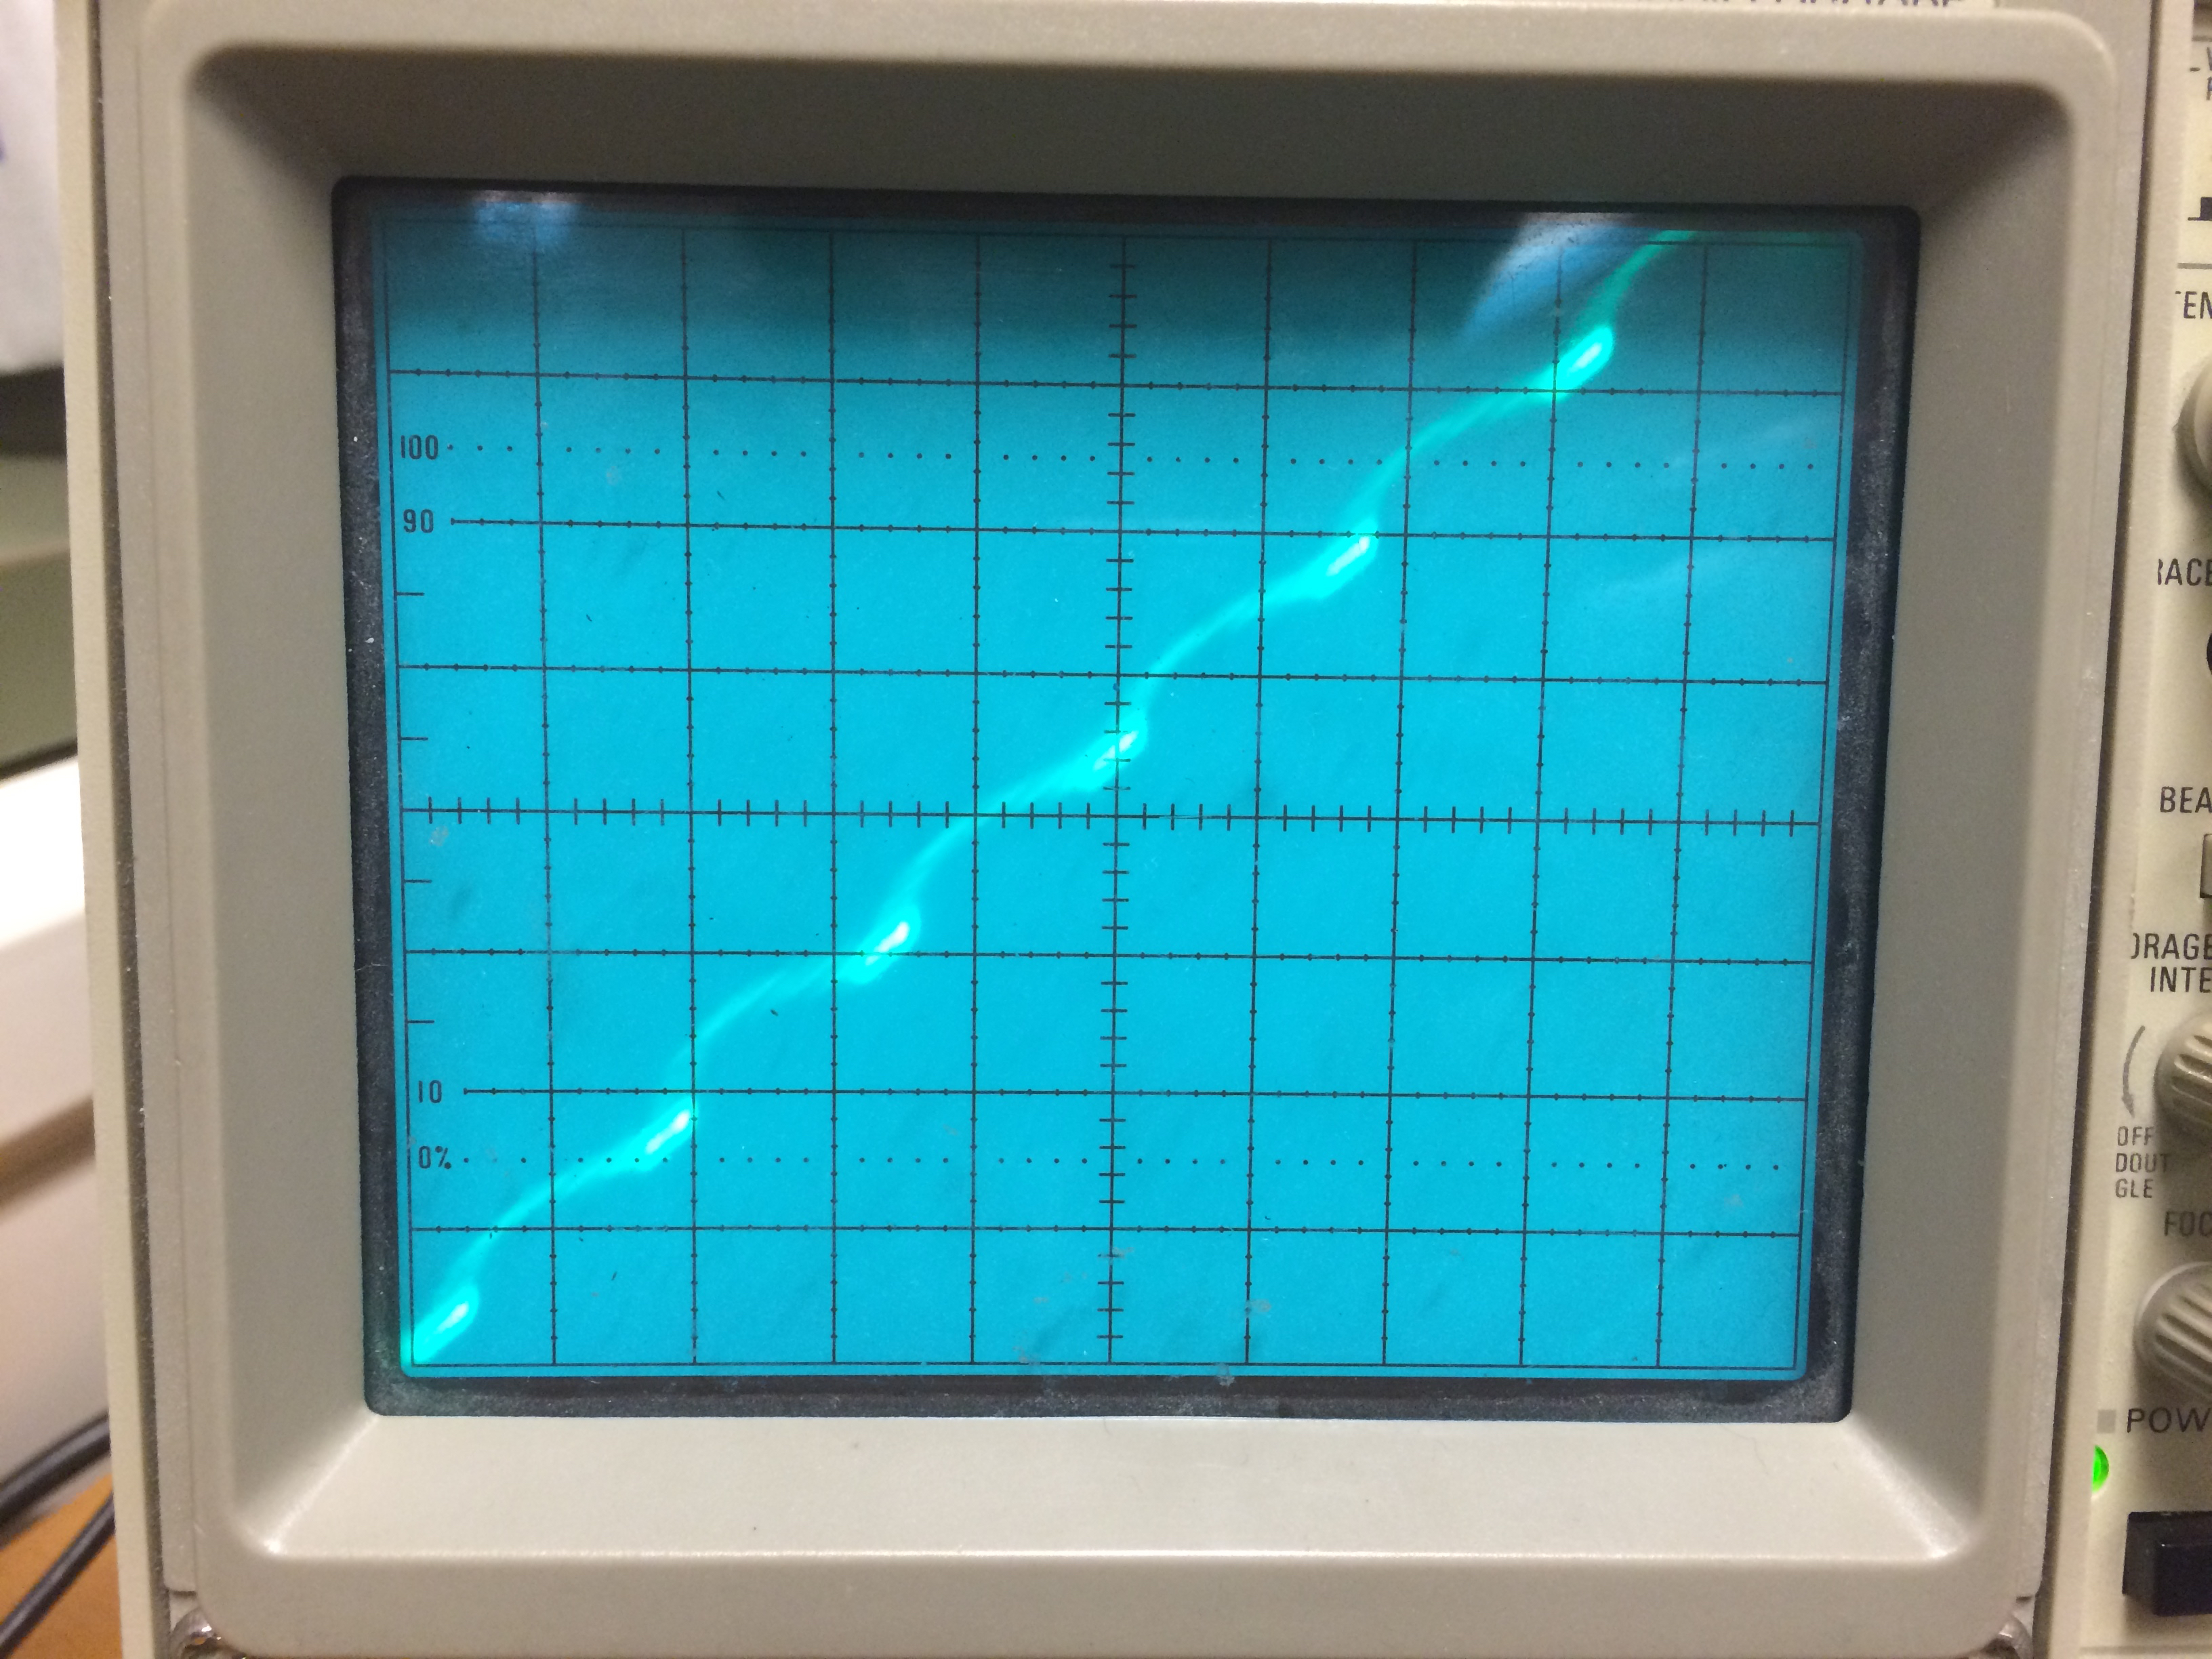
\includegraphics[height=0.4\textheight]{images/dots_x8.jpg}
        \caption{Zooming in eight times, we can also observe that the electron ray do not move in a straight line from point to point.}
        \label{fig:dotx8}
    \end{subfigure}
    \caption{A diagonal line with different levels of zoom}
    \label{fig:artefact-dots}
\end{figure}

\subsection{HDMI}
Rasterisation and HDMI was not implemented.
The intention of this part was to demonstrate the difference between vector and raster output in real-time.
However this parts of the system was no longer prioritized when the analogue counterpart proved to be a reliable source of output.
Moreover, this part was a medium priority requirement, listed in Table \ref{tbl:non_func_req}, and thus not a critical part of \vthreek 

\section{Budget}
In the assignment text the group was given a budget of 10,000 NOK.
At the end of the project the total cost of materials was 11,504.25NOK (without shipping costs), which is somewhat above the proposed budget for the project.
The full list of material expenses is listed in Appendix \ref{tbl:material-cost}.